\documentclass[11pt]{article}
\usepackage[margin=1in]{geometry}
\usepackage{amsmath,amssymb,graphicx,listings,xcolor,float}
\usepackage{enumitem}
\usepackage{epstopdf}

\lstset{
  language=Matlab,
  basicstyle=\small\ttfamily,
  keywordstyle=\color{blue},
  commentstyle=\color{green!50!black},
  stringstyle=\color{red},
  numbers=left,
  numberstyle=\tiny\color{gray},
  breaklines=true,
  frame=single,
  tabsize=4
}

\title{MATH 543 -- Homework 7}
\author{Parham Khodadi}
\date{}\begin{document}
\maketitle

%% ============================================================
\section*{Intro}
%% ============================================================

Use Gaussian Elimination with Partial Pivoting (GE w/PP) to study the growth factor (Eq. 22.2):
\[\rho = \frac{\max_{i,j} |u_{ij}|}{\max_{i,j} |a_{ij}|}\]
by creating plots analogous to TB-Figure 22.1 and TB-Figure 22.2. For computational efficiency, use the built-in \texttt{lu()} factorization with partial pivoting.

\begin{figure}[H]
    \centering
    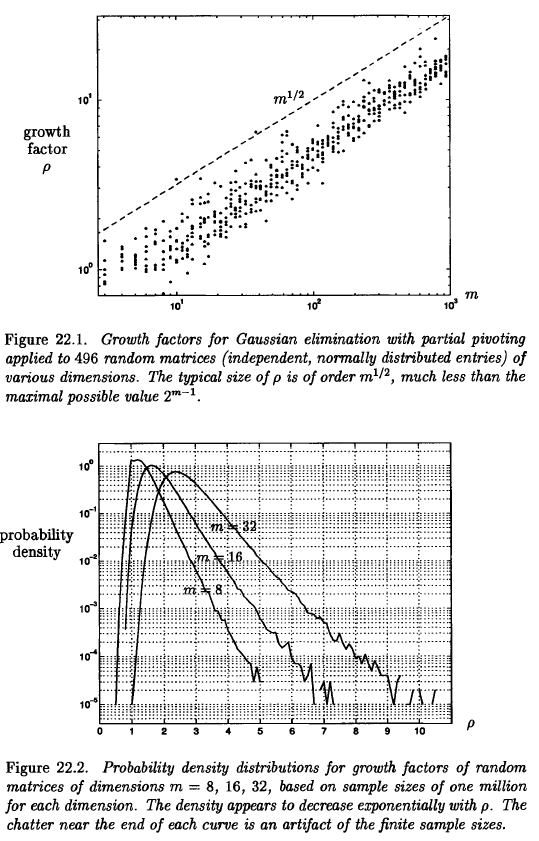
\includegraphics[width=0.58\linewidth]{TB.png}
\end{figure}

%% ============================================================
\newpage
\section*{6.5.1}
%% ============================================================

\subsection*{Problem}
For matrices with random, normally distributed $N(0,1)$ entries, plot the growth factor $\rho$ for GE w/PP. (TB-Figure 22.1) --- Use at least 1,024 matrices with varying sizes (up to at least $2048 \times 2048$ matrices).

\subsection*{Solution}
MATLAB code found in Appendix.

\begin{figure}[H]
    \centering
    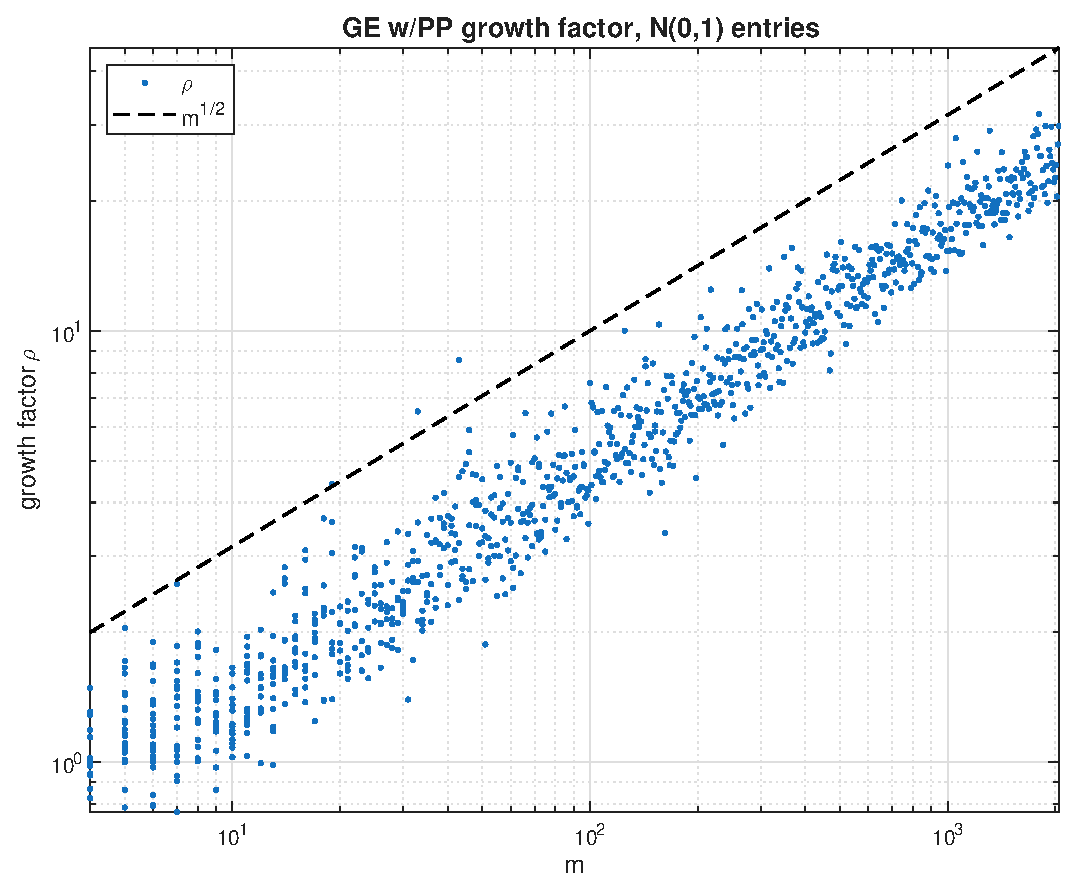
\includegraphics[width=1\textwidth]{Figures/P6_5_1.eps}
    \caption{Growth factor $\rho$ for GE w/PP applied to random $N(0,1)$ matrices of varying size $m$.}
    \label{fig:6_5_1}
\end{figure}


%% ============================================================
\newpage
\section*{6.5.2}
%% ============================================================

\subsection*{Problem}
For matrices with random, normally distributed $N(0,1)$ entries, plot the probability density of $\rho$. (TB-Figure 22.2) --- Use at least 1,048,576 matrices of each $m \times m$ size, $m \in \{8, 16, 32, 64\}$.

\subsection*{Solution}
MATLAB code found in Appendix.

\begin{figure}[H]
    \centering
    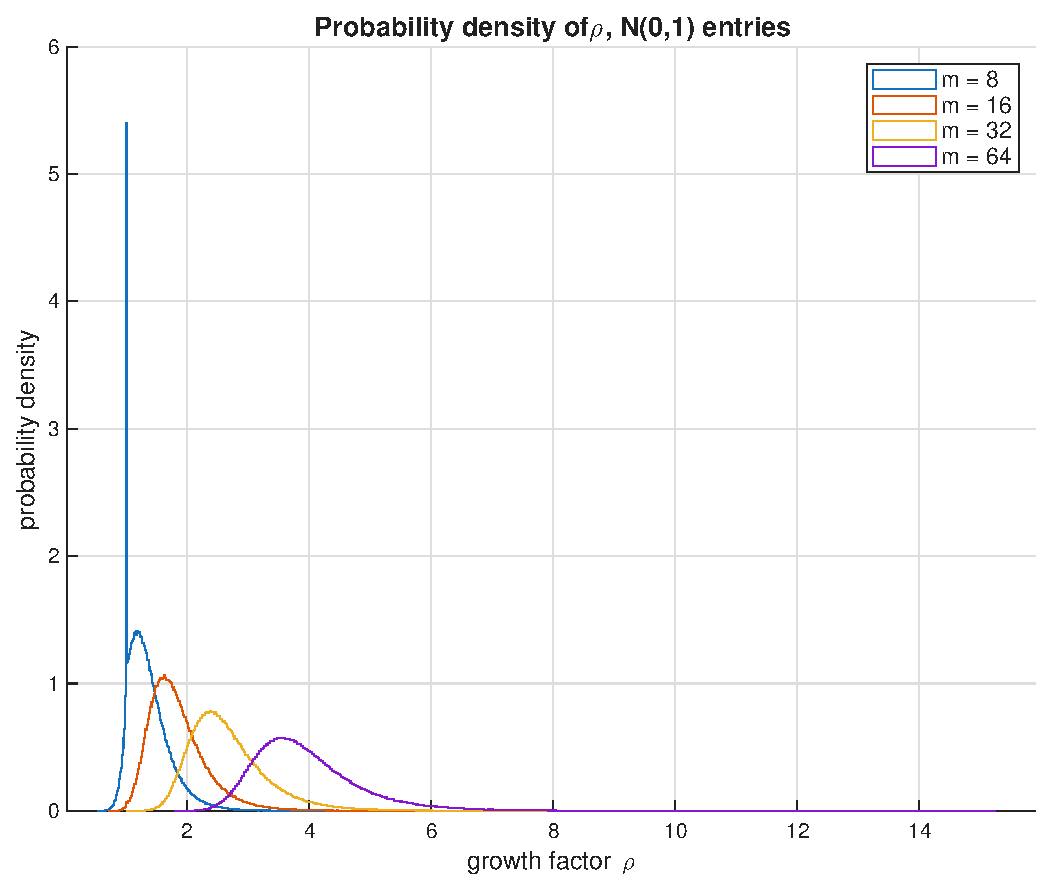
\includegraphics[width=1\textwidth]{Figures/P6_5_2.eps}
    \caption{Probability density of growth factor $\rho$ for $N(0,1)$ matrices with $m \in \{8, 16, 32, 64\}$.}
    \label{fig:6_5_2}
\end{figure}


%% ============================================================
\newpage
\section*{6.5.3}
%% ============================================================

\subsection*{Problem}
For matrices with random, uniformly distributed entries in $[0,1]$, plot the growth factor $\rho$ for GE w/PP as a function of matrix size $m$ (variant of TB-Figure 22.1). Use at least 1,024 matrices with varying sizes (up to at least $2048 \times 2048$ matrices).

\subsection*{Solution}
MATLAB code found in Appendix.

\begin{figure}[H]
    \centering
    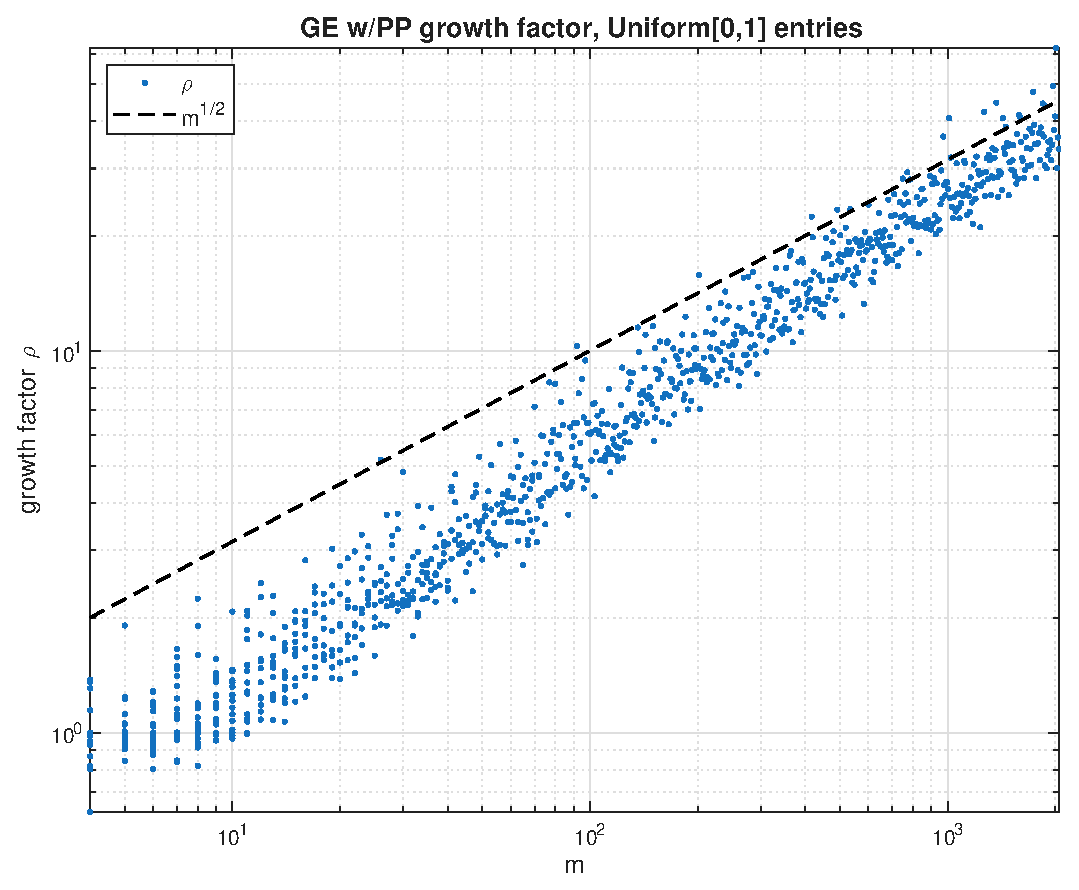
\includegraphics[width=1\textwidth]{Figures/P6_5_3.eps}
    \caption{Growth factor $\rho$ for GE w/PP applied to random uniform $[0,1]$ matrices of varying size $m$.}
    \label{fig:6_5_3}
\end{figure}


%% ============================================================
\newpage
\section*{6.5.4}
%% ============================================================

\subsection*{Problem}
For matrices with random, uniformly distributed entries in $[0,1]$, plot the probability density of the growth factor $\rho$ (variant of TB-Figure 22.2). Use at least 1,048,576 matrices of each $m \times m$ size, $m \in \{8, 16, 32, 64\}$.

\subsection*{Solution}
MATLAB code found in Appendix.

\begin{figure}[H]
    \centering
    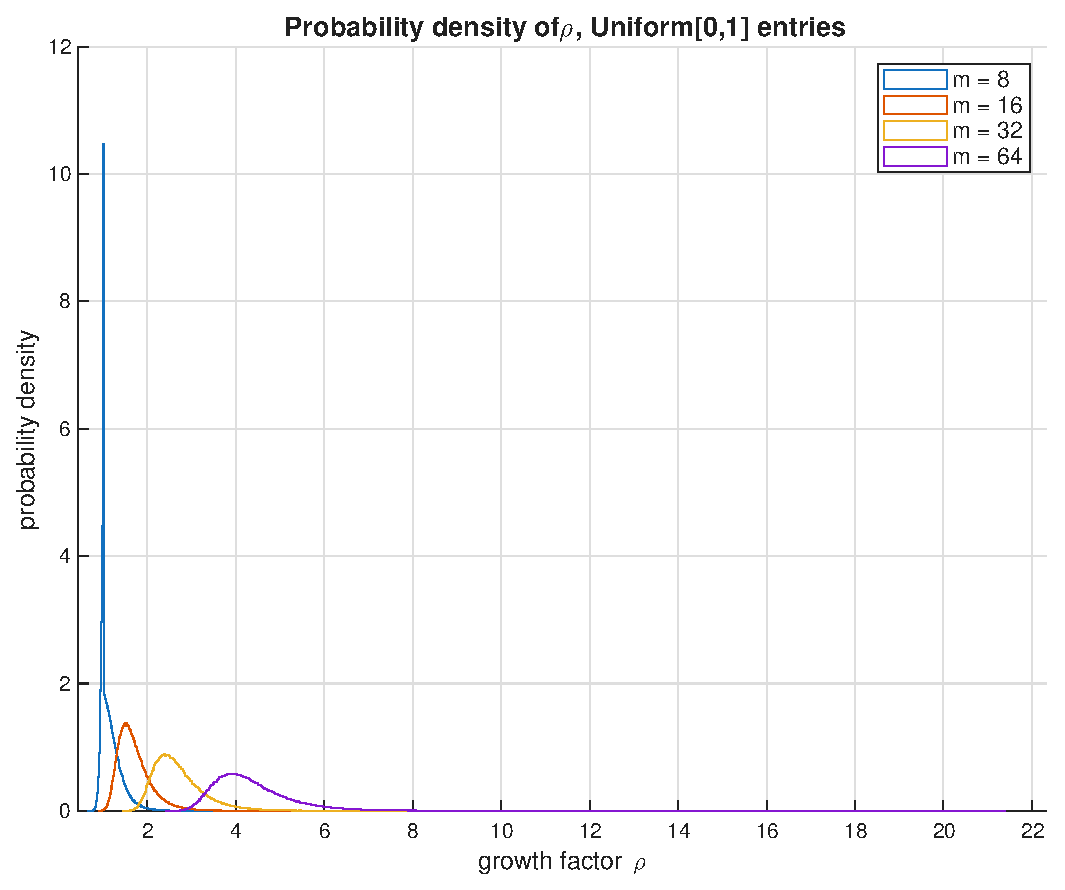
\includegraphics[width=1\textwidth]{Figures/P6_5_4.eps}
    \caption{Probability density of growth factor $\rho$ for uniform $[0,1]$ matrices with $m \in \{8, 16, 32, 64\}$.}
    \label{fig:6_5_4}
\end{figure}


%% ============================================================
\newpage
\section*{6.5.5}
%% ============================================================

\subsection*{Problem}
Comment on similarities and differences of normally distributed $N(0,1)$ vs. uniformly distributed $[0,1]$ matrix entries.

\subsection*{Discussion}
\subsubsection*{Similarities}
Figures 1 and 3 are visually almost the same plot. In both, the cloud of $\rho$ values rides along and just below the dashed $\sqrt{m}$ line across the full range $m \in [4, 2048]$, and in both the largest observed $\rho$ at $m = 2048$ is only around 30–40, which is nowhere near the worst-case $2^{m-1}$ from Lecture 17.

Figures 2 and 4 also share the same shape. For each $m$ the density has a peak near small $\rho$ and a right tail that decays fast, and as $m$ grows the peak shifts right and the distribution broadens. Both entry distributions confirm that $\rho \approx \sqrt{m}$ is practically stable.

\subsubsection*{Differences}
Comparing Figures 2 and 4 directly, the uniform case produces slightly more spread. The right tails in Figure 4 extend out to roughly $\rho \approx 22$ for $m = 64$, while Figure 2's tails stop near $\rho \approx 14$. The $m = 64$ mode sits near $\rho \approx 4$ for uniform entries but near $\rho \approx 3.5$ for Gaussian entries. That is a small but visible rightward shift. 

%% ============================================================
\newpage
\section*{Appendix: MATLAB Code}
%% ============================================================

\lstinputlisting{HW7.m}

\end{document}